\documentclass[conference]{IEEEtran}
\usepackage{amsmath,amssymb}
\usepackage{booktabs}
\usepackage{array}
\usepackage{xcolor}
\usepackage{url}
\usepackage[hidelinks]{hyperref}
\usepackage{cite}
\usepackage{tikz}
\usetikzlibrary{positioning,arrows.meta}

\renewcommand{\topfraction}{0.9}
\renewcommand{\dbltopfraction}{0.9}
\renewcommand{\textfraction}{0.05}
\renewcommand{\floatpagefraction}{0.8}
\renewcommand{\dblfloatpagefraction}{0.8}

\newcommand{\TODO}[1]{\textcolor{red}{\textbf{[TODO: #1]}}}
\newcommand{\Accept}{\mathrm{Accept}}
\newcommand{\ValidCont}{\mathrm{ValidCont}}
\newcommand{\PoR}{\mathrm{PoR}}
\newcommand{\PoC}{\mathrm{PoC}}
\newcommand{\Priv}{\mathrm{Priv}}
\newcommand{\scope}{\mathrm{scope}}
\newcommand{\aud}{\mathrm{aud}}
\newcommand{\Comp}{\mathrm{Comp}}
\newcommand{\Hsh}{\mathsf{H}}
\newcommand{\X}{\mathcal{X}}
\newcommand{\Lin}{\mathcal{L}}

\newtheorem{definition}{Definition}
\newtheorem{lemma}{Lemma}
\newtheorem{theorem}{Theorem}
\newtheorem{proposition}{Proposition}
\newtheorem{corollary}{Corollary}
\newtheorem{assumption}{Assumption}
\newtheorem{remark}{Remark}

\begin{document}

\title{Provenance Is Not Continuity:\\Execution-Context Non-Mixing as a Protocol Invariant for Authority Propagation under Untrusted Execution}

\author{\IEEEauthorblockN{\TODO{Author(s)}}
\IEEEauthorblockA{\TODO{Affiliation}}}

\maketitle

\begin{abstract}
Authority in distributed systems is created by authentication and authorization protocols such as OpenID Connect and OAuth~2.0, and is then \emph{propagated} across execution boundaries: services, workloads, tools, and AI agents. We examine one narrowly defined property of propagation, \emph{execution-context non-mixing}: a receiving boundary must accept propagated authority only as the continuation of the one concrete execution occurrence from which it descends. We start from the strongest token-based propagation baseline available today---an authorization server issuing DPoP-bound tokens with strict scope attenuation at every exchange, audience restriction, and policy-approved composition of independent lineages---and formalize the inputs its receivers read. We prove that these inputs are \emph{execution-invariant}: two occurrences of the same grant, at the same executor, for the same operation and resource, are indistinguishable to a conformant receiver, so mixing authority across concurrent executions is \emph{conformant} behaviour of the baseline rather than a defect of any implementation. We further show that self-asserted execution identifiers do not remove the gap, because the executor's assertion is not evidence. We then show that the gap is closed by adding a single conjunct to the receiving predicate---receiver-verifiable evidence binding each step to its specific predecessor and, where the profile requires it, to the signed request, together with non-expansive authority---and prove that the resulting predicate, Provenance Identity Continuity (PIC), establishes non-mixing under stated cryptographic and verification assumptions. We position the result relative to attenuation-chain systems (Macaroons, Biscuit), named-delegate systems (UCAN, SPKI/SDSI), and OAuth token exchange, distinguishing what each can do optionally, what each cannot do without becoming a continuity verifier, and what PIC makes mandatory. We instantiate the gap for long-running, concurrent AI agents and state precisely which failures PIC does and does not prevent, and we demonstrate both results on running software: a conformant Keycloak-issued, DPoP-bound baseline accepts the mixed presentation with every check passing, while under PIC-X, an implementation of the Profile~0.2 exchange, every misattributed presentation is rejected with the failing conjunct named, valid authority is accepted only under its own occurrence, and the resulting attribution supports receiver policies over occurrences that the baseline cannot express.
\end{abstract}

\begin{IEEEkeywords}
Authorization, authority propagation, confused deputy, OAuth 2.0, DPoP, capabilities, AI agents.
\end{IEEEkeywords}

\section{Introduction}\label{sec:intro}

Consider a deployment that does everything current practice recommends. A user authenticates through OpenID Connect. An authorization server (AS) issues an OAuth~2.0 access token bound to the client's key with DPoP~\cite{rfc9449}. At every downstream hop the token is exchanged~\cite{rfc8693} for a new one whose scope is a subset of the previous scope and whose audience is the next service~\cite{rfc8707}. When two independent workflows must act together, a policy explicitly approves their joint participation while keeping them distinct. Every artifact is authentic, every scope is attenuated, every presenter controls the required key.

Now let the executor at some hop be an AI agent that serves two requests from the same user concurrently. Request~$A$ authorizes \texttt{write}; request~$B$ authorizes \texttt{read}. The agent holds two valid tokens. While processing request~$B$ it presents the token issued for request~$A$. Every check listed above passes. The receiving service performs a write that request~$B$ never authorized, and no participant violated any specification.

This paper is about that gap. It is not a gap in authentication, in consent, or in the creation of authority: those are handled by OIDC and OAuth, and we presuppose them. It is a gap in \emph{propagation}. A valid delegation chain establishes \emph{provenance}---where authority came from. Attenuation establishes \emph{non-expansion}. Holder binding establishes \emph{control of a key}. Composition establishes \emph{what may participate together}. None of these establishes which concrete execution the authority is allowed to \emph{continue}. We call that missing property \emph{continuity}, and we show that it is not a matter of implementation quality: the receiver's inputs, as specified, contain no evidence that could distinguish the two executions.

Non-mixing is an attribution property, and we state at the outset what it does and does not buy in the opening scenario. Under $\mathbf{P}$ the agent can still exercise request~$A$'s \texttt{write} while doing request~$B$'s work: that presentation is a valid continuation of $X_A$ and is accepted \emph{as $X_A$} (run P8, \S\ref{sec:impl}). What changes is that the accepted state now names its occurrence. Three consequences follow, each observed in \S\ref{sec:impl}: the union of the two authorities is unrepresentable; a presentation of one occurrence's authority \emph{as the continuation of the other} is rejected; and a receiver can bind a workflow to the occurrence that started it and refuse continuations of any other (run P9)---a policy the baseline cannot express at all, because its receiver inputs carry no occurrence (Lemma~\ref{lem:invariance}). Whether an operation accepted under its true occurrence serves the purpose of that occurrence's request remains semantic intent, outside the property (\S\ref{sec:limits}).

\subsubsection*{Contributions}
\begin{enumerate}
\item A formal separation between an \emph{execution occurrence} $X$, its \emph{provenance} $D(X)$, and the \emph{inputs} $T$ a receiving boundary reads (\S\ref{sec:setting}).
\item A lemma showing, field by field, that the inputs read by a receiver under the strongest token baseline---including every DPoP proof field---are execution-invariant (\S\ref{sec:baseline}, Lemma~\ref{lem:invariance}), and a theorem showing that the baseline therefore cannot establish execution-context non-mixing while behaving in full conformance (Theorem~\ref{thm:gap}).
\item A lemma showing that self-asserted execution identifiers do not close the gap (Lemma~\ref{lem:selfasserted}).
\item A receiving predicate obtained by adding one conjunct to the baseline, $\Accept_{\mathrm{PIC}} = \Accept_{B} \wedge \PoR \wedge \subseteq$, and a conditional sufficiency theorem (\S\ref{sec:pic}, Theorem~\ref{thm:sufficiency}), together with explicit treatment of duplicate delivery, composition, and deferred outcomes.
\item A three-tier comparative result: token exchange cannot establish the property without becoming a continuity verifier; attenuation-chain systems can establish it as an optional deployment discipline; PIC makes it mandatory (\S\ref{sec:comparison}).
\item An instantiation for AI agents stating exactly what PIC prevents and what it does not (\S\ref{sec:agents}), and an integration path from OAuth~2.0 origination to PIC propagation (\S\ref{sec:oauth}).
\item An experimental demonstration on running software (\S\ref{sec:impl}): a conformant OAuth~2.0 + DPoP deployment (Keycloak) accepting the mixed presentation with every receiver check passing; every misattributed presentation rejected by PIC-X~\cite{picx}, an implementation of the Profile~0.2 exchange, with the failing conjunct named; the honest cross-occurrence use accepted under its own occurrence; and a receiver-side occurrence policy, inexpressible under the baseline, enforced on the attribution.
\end{enumerate}

This paper extends the model introduced in~\cite{gallo2026poc}. Relative to that work, the following are new: the occurrence/provenance/receiver-input separation (Defs.~\ref{def:occurrence}--\ref{def:inputs}), property $\mathbf{P}$ stated over receiver inputs (Def.~\ref{def:P}), the field-level invariance lemma for the concrete baseline (Lemma~\ref{lem:invariance}), the conformance claim of Theorem~\ref{thm:gap}, the self-asserted-discriminator lemma (Lemma~\ref{lem:selfasserted}), the complement equation (Def.~\ref{def:acceptpic}), the treatment of $\mathbf{U}$ (Prop.~\ref{prop:dup}) and composition (Prop.~\ref{prop:compose}), the three-tier comparison (\S\ref{sec:comparison}), and the experimental demonstration (\S\ref{sec:impl}). The following restate or specialize~\cite{gallo2026poc}: Def.~\ref{def:invariant} generalizes lineage-invariant authorization~\cite[Defs.~7--8]{gallo2026poc} from privilege sets to receiver inputs; Defs.~\ref{def:por}--\ref{def:poc} restate PoR, valid transition, and PoC~\cite[Defs.~4--6]{gallo2026poc} in the concrete Profile~0.2 construction; Theorem~\ref{thm:sufficiency} is the concrete counterpart of PIC safety, origin binding, and confused-deputy impossibility~\cite[Thm.~1, Lem.~1, Thm.~6]{gallo2026poc}; Cor.~\ref{cor:mixing} is the receiver-input counterpart of~\cite[Thm.~6]{gallo2026poc}; and Lemma~\ref{lem:selfasserted} strengthens~\cite[Thm.~4]{gallo2026poc} by requiring the separating lineage function to be authenticated rather than merely present.

\section{Threat Model and Evaluation Method}\label{sec:threat}

The threat model is defined for this paper and is the perimeter against which every mechanism below, including PIC, is evaluated.

\subsection{Untrusted execution}
An executor is \emph{untrusted} when the security argument may not assume that its internal behaviour preserves correct request-to-authority attribution. This covers defects, compromise, prompt injection, non-deterministic authority selection, retained state, and execution across boundaries that do not themselves prove which request an authority state belongs to. The classification concerns what a proof may assume; it is not an allegation about any implementation. Long-running AI agents are the motivating instance: they serve overlapping requests, hold several authority sources at once, and select later tools, services, or agents at runtime. The threat model refuses to use the agent's internal correctness as the proof presented to the next boundary.

\subsection{Elements}
\begin{enumerate}
\item[\textbf{T1}] \textbf{Transport is untrusted.} Channel location, routing, or possession of an artifact is not proof that authority belongs to the execution being continued. Conforming deployments still use TLS; TLS protects the channel, not the attribution.
\item[\textbf{T2}] \textbf{Execution is untrusted and there is no required global mediator.} The executor's internal choice is not accepted as proof of attribution, and the model does not require a separate globally trusted component to separate execution steps. Each receiving boundary still performs trusted verification and enforcement.
\item[\textbf{T3}] \textbf{Execution may overlap or retain state.} Independent requests and authority contexts coexist, interleave, or remain available after an earlier step. Concurrency is the principal case; retained state creates the same question sequentially.
\item[\textbf{T4}] \textbf{The $N{+}1$ unidentified successor.} A concrete successor may not exist or be identifiable when authority is originated. Eligibility may be defined in advance; the concrete successor is evaluated when it materializes.
\item[\textbf{T5}] \textbf{The $N{+}1$ invalid authority state.} A receiver must reject a successor state that expands the authenticated predecessor context or presents authority from one execution as the continuation of another. The executor's own selection is not the proof.
\end{enumerate}

\subsection{Evaluation method}
A protocol guarantee consists of what its model represents and what a conforming receiver verifies. (P1)~Authority already exists; the subject is propagation. (P2)~A guarantee must follow from represented state, transition rules, acceptance predicates, and explicit assumptions---not from the expectation that executors behave. (P3)~Dependencies on scheduler behaviour, request routing, memory separation, executor cooperation, or a global mediator are assumptions and remain attack surface unless separately modelled. (P4)~Closure is property-specific. (P5)~Local conduct and propagated acceptance are different questions: no authorization protocol proves that an executor's local actions are semantically correct; the protocol question is whether one executor can cause a later conforming boundary to accept authority invalid for the represented continuation.

\subsection{Adversary}
The adversary may influence requests, payloads, parameters, and an executor's authority selection; may control executors entirely; may read, copy, delay, reorder, drop, or replay messages. The adversary cannot break the underlying cryptography, cannot compromise the verifier at a conforming receiving boundary, and cannot compromise the origination of authority (the AS) or the attestation issuers. These exclusions apply equally to every mechanism compared.

\section{Formal Setting}\label{sec:setting}

Let $P$ be a set of principals, $O$ a set of operations, $R$ a set of resources. A privilege is $(o,r)\in O\times R$; an \emph{authority context} is $C\subseteq O\times R$. Each principal $p$ has $\Priv(p)\subseteq O\times R$.

\begin{definition}[Execution occurrence]\label{def:occurrence}
An \emph{execution occurrence} $X$ is one concrete run originated by one signed request $\rho(X)$ from a principal $p(X)$ with origin authority context $C_0(X)\subseteq\Priv(p(X))$. Its lineage is a finite sequence of steps $\ell(X)=\langle s_0,\dots,s_n\rangle$ with $s_i\prec s_{i+1}$, each carrying $C_i(X)$. $\X$ denotes the set of occurrences.
\end{definition}

Two occurrences may have the same principal, executor, operation, resource, and privilege set and remain distinct: $C_A=C_B \not\Rightarrow X_A=X_B$.

\begin{definition}[Provenance]\label{def:provenance}
The \emph{provenance} $D(X)$ of the authority held at a step is the sequence of authority artifacts (tokens, certificates, capabilities) by which that authority reached the step, with their issuers, subjects, scopes, audiences, and holder bindings. $D$ answers \emph{where the authority came from}.
\end{definition}

\begin{definition}[Presentation and receiver inputs]\label{def:inputs}
A \emph{presentation} $\sigma=(\tau,\pi,q)$ consists of an authority artifact $\tau$, an accompanying proof $\pi$ (e.g.\ a DPoP proof), and the concrete request $q$. A receiving boundary computes an input tuple $T(\sigma)$ from $\sigma$ and its local state and applies an acceptance rule $A:\mathrm{Range}(T)\to\{0,1\}$. $S(\sigma)\subseteq O\times R$ denotes the authority the presentation claims.
\end{definition}

\begin{definition}[Valid continuation]\label{def:validcont}
$\ValidCont(S,X)$ holds iff $S$ is bound by verified evidence to one specific step $s_i$ of $\ell(X)$ and $S\subseteq C_i(X)$.
\end{definition}

\begin{definition}[Execution-context non-mixing, property $\mathbf{P}$]\label{def:P}
A receiving rule \emph{establishes} $\mathbf{P}$ iff every accepted presentation $\sigma$ satisfies:
\begin{enumerate}
\item[(i)] \emph{uniqueness}: $\sigma$ identifies, by verified evidence, exactly one origin occurrence $X(\sigma)$;
\item[(ii)] \emph{boundedness}: $S(\sigma)\subseteq C_0(X(\sigma))$;
\item[(iii)] \emph{predecessor specificity}: $S(\sigma)$ is bound to one specific predecessor step of $\ell(X(\sigma))$ and $S(\sigma)\subseteq C_i(X(\sigma))$ at that step.
\end{enumerate}
Consequently, if $S_B\not\subseteq C_i(X_A)$, a presentation of $S_B$ as a continuation of $X_A$ is rejected, and no accepted state draws authority from two occurrences.
\end{definition}

$\mathbf{P}$ is an authority property. It does not assert that the operation performed under $X$ serves the purpose of $\rho(X)$ (semantic intent), and it does not track the flow of data. \S\ref{sec:limits} returns to both.

\begin{definition}[Execution-invariant receiving rule]\label{def:invariant}
A receiving rule is \emph{execution-invariant} if $T(\sigma)$ is determined by $(\tau,\pi,q)$ and local receiver state and contains no component whose value is bound, by evidence the presenter cannot self-assert, to the occurrence that $\sigma$ purports to continue. Equivalently, writing $e=(S,X)$ and $p(e)=S$, there is $\bar A$ with $A=\bar A\circ p$.
\end{definition}

This generalizes the lineage-invariant authorization of~\cite[Defs.~7--8]{gallo2026poc} from privilege sets to receiver inputs.

\section{The Strongest Token Baseline and Its Execution-Invariance}\label{sec:baseline}

\subsection{Baseline $B$}
We fix the most demanding token-based propagation stack that current specifications support, so that the gap we exhibit cannot be attributed to a weak target.

\begin{enumerate}
\item[\textbf{B1}] \textbf{Origination.} The AS issues, after OIDC authentication and OAuth consent, an access token $\tau_0$ with claims $\mathrm{sub},\aud,\scope,\mathrm{exp}$ and a confirmation claim $\mathrm{cnf}$ carrying the thumbprint of the client's DPoP key~\cite{rfc9449,rfc7519}.
\item[\textbf{B2}] \textbf{Strict attenuation at every exchange.} At each hop the current executor exchanges $\tau_i$ for $\tau_{i+1}$~\cite{rfc8693}; the AS enforces $\scope(\tau_{i+1})\subseteq\scope(\tau_i)$ and sets $\aud(\tau_{i+1})$ to the next service~\cite{rfc8707}. The AS may record the delegation history in an \texttt{act} chain.
\item[\textbf{B3}] \textbf{Holder binding per request.} Every presentation carries a DPoP proof $\pi$ signed by the key in $\mathrm{cnf}(\tau)$, with fields $\mathrm{jti},\mathrm{htm},\mathrm{htu},\mathrm{iat},\mathrm{ath}=\Hsh(\tau)$, and, when the receiver demands it, a server-provided $\mathrm{nonce}$~\cite{rfc9449}.
\item[\textbf{B4}] \textbf{Explicit composition.} When two independent lineages $L_1,L_2$ must participate jointly, a policy $\Comp(L_1,L_2)\in\{\mathrm{approve},\mathrm{deny}\}$ is evaluated; approval does not merge the two token sets.
\end{enumerate}

The receiver's input tuple is
\begin{align*}
T_B(\sigma) = \big(&\mathrm{sig}(\tau),\ \mathrm{exp}(\tau),\ \aud(\tau)\overset{?}{=}\mathrm{self},\\
&(o,r)\in\scope(\tau),\ \mathrm{sig}_{\mathrm{cnf}(\tau)}(\pi),\\
&\mathrm{htm}(\pi)\overset{?}{=}\mathrm{method}(q),\ \mathrm{htu}(\pi)\overset{?}{=}\mathrm{uri}(q),\\
&\mathrm{ath}(\pi)\overset{?}{=}\Hsh(\tau),\ \mathrm{jti}(\pi)\ \mathrm{fresh},\\
&\mathrm{nonce}(\pi)\ \mathrm{valid},\ \Comp\big).
\end{align*}

\subsection{Execution-invariance of $T_B$}

\begin{lemma}[$T_B$ is execution-invariant]\label{lem:invariance}
Let $E$ be an executor hosting two occurrences $X_A\neq X_B$ on behalf of the same principal, holding tokens $\tau_A,\tau_B$ issued under $B$, and let $R$ be a receiver to which both occurrences would continue with the same $(o,r)$. For any token $\tau\in\{\tau_A,\tau_B\}$ and any fresh proof $\pi$ for $\tau$, every component of $T_B(\tau,\pi,q)$ takes the same value whether $q$ continues $X_A$ or $X_B$.
\end{lemma}

\begin{IEEEproof}
Component by component. $\mathrm{sig}(\tau)$, $\mathrm{exp}(\tau)$, $\aud(\tau)$, $\scope(\tau)$ are properties of the artifact $\tau$ and do not mention $X$. $\mathrm{sig}_{\mathrm{cnf}(\tau)}(\pi)$ verifies under a key determined by $\tau$; $E$ holds that key in both occurrences. $\mathrm{htm}$ and $\mathrm{htu}$ are determined by the operation and the receiver, which coincide by hypothesis. $\mathrm{ath}$ binds $\pi$ to $\tau$, not $\tau$ to $X$: it equals $\Hsh(\tau)$ for whichever $\tau$ is presented. $\mathrm{jti}$ is chosen by $E$ and is fresh in both cases. $\mathrm{nonce}$ is chosen by $R$ to bound the proof's age; it is issued before $R$ knows anything about $X$ and is therefore not a function of $X$. $\Comp$ is a function of the participating lineage sets, not of which occurrence is being continued. No component's value is bound by evidence to $X$; hence $T_B$ factors through the projection that forgets $X$ (Def.~\ref{def:invariant}).
\end{IEEEproof}

\begin{remark}
Lemma~\ref{lem:invariance} does not say that DPoP is not request-bound. It is: $\pi$ is bound to the HTTP method, URI, token, and freshness window. It says that none of those bindings is a binding to the \emph{predecessor execution}. Two occurrences of the same grant produce different proofs with identical decision-relevant content.
\end{remark}

\begin{theorem}[Gap]\label{thm:gap}
$B$ does not establish $\mathbf{P}$. Moreover, the violating execution is conformant: the AS behaves in accordance with~\cite{rfc6749,rfc8693}, the receiver in accordance with~\cite{rfc6750,rfc9449}, and no artifact is forged, expanded, or replayed.
\end{theorem}

\begin{IEEEproof}
Take $E$, $X_A$, $X_B$, $\tau_A$, $\tau_B$ as in Lemma~\ref{lem:invariance} with $\scope(\tau_A)\not\subseteq C_0(X_B)$. Let $E$, while processing the request $q_B$ that continues $X_B$, present $\sigma=(\tau_A,\pi_A,q_B)$ with a fresh valid $\pi_A$. By Lemma~\ref{lem:invariance}, $T_B(\sigma)$ equals the tuple that would be computed for the legitimate presentation of $\tau_A$ within $X_A$; the acceptance rule, being a function of $T_B$, accepts. The accepted state $S(\sigma)=\scope(\tau_A)$ is not a valid continuation of $X_B$ (Def.~\ref{def:validcont}), so (ii) of $\mathbf{P}$ fails; (i) fails because $\tau_A$ identifies a \emph{grant}, of which $X_A$ and $X_B$ are two occurrences, not an occurrence. Every step is conformant: the AS issued $\tau_A$ correctly, the receiver validated it correctly, $E$ controlled the key it was required to control.
\end{IEEEproof}

The last sentence is the substantive point. Tokens individuate \emph{grants}; the property requires individuating \emph{occurrences}. The mismatch is not a defect to be fixed in an implementation; a perfectly implemented $B$ exhibits it. \S\ref{sec:impl} shows the accepting run on a conformant deployment (run B1): every receiver check of $T_B$, including all DPoP proof fields, passes on the mixed presentation.

\subsection{Self-asserted discriminators do not close the gap}

An apparent remedy is to add an execution identifier to the token.

\begin{lemma}[Self-asserted discriminators]\label{lem:selfasserted}
Extend $B$ so that at each exchange the requesting executor supplies a claim $\mathrm{exec\_id}$ that the AS copies into $\tau_{i+1}$, and receivers check that $\mathrm{exec\_id}(\tau)$ matches the execution they believe they are serving. The extended rule still does not establish $\mathbf{P}$.
\end{lemma}

\begin{IEEEproof}
For the mixing request, $E$ requests an exchange of $\tau_A$ while asserting $\mathrm{exec\_id}=\mathrm{id}(X_B)$. Under the extended $B$ the AS verifies $\tau_A$, attenuates the scope, and copies the asserted identifier; it has no input against which to verify that $\tau_A$ belongs to $X_B$. The resulting token carries $\scope(\tau_A)$ and $\mathrm{exec\_id}=\mathrm{id}(X_B)$. The receiver's check passes. The value of the new component is determined by $E$'s assertion, hence is not bound by evidence to $X$ (Def.~\ref{def:invariant}); the extended $T$ remains execution-invariant in the sense required.
\end{IEEEproof}

\begin{remark}
The AS \emph{could} verify the asserted identifier: by requiring the exchange request to present the predecessor token issued within $X_B$ and checking that the requested scope is a subset of that predecessor's scope. That check is a verification of a predecessor relation and of non-expansion relative to it; it is the primitive of \S\ref{sec:pic}, performed by the AS rather than by the receiver. Theorem~4 of~\cite{gallo2026poc} states the general form: any rule that separates two occurrences with equal projection must read an authenticated function of the occurrence. What Lemma~\ref{lem:selfasserted} adds is that the function must be \emph{authenticated}, not merely present.
\end{remark}

\subsection{A reachable interleaving}
The failure does not require a malicious executor. Let $E$ maintain a shared authority accumulator that composes incoming contexts by union and is cleared when a call completes. Under sequential processing, call~1 executes with $C_A$ and call~2 with $C_B$. Under the interleaving \emph{receive~$A$, receive~$B$, execute~2, execute~1}, both calls execute with $C_A\cup C_B$; call~1 may exercise $b\in C_B\setminus C_A$ and call~2 may exercise $a\in C_A\setminus C_B$. Every input is authentic and every privilege was granted by the same principal. The accumulator is a countermodel, not a characterization of any implementation category; its purpose is to show that the violating state is reachable under T3 without intent. Run~B1b of \S\ref{sec:impl} executes exactly this interleaving.

\begin{definition}[Temporal confused deputy]\label{def:tcd}
An accepted transition in which the presented authority is valid with respect to its operation-and-resource projection but is not validly attributable to the execution occurrence under which it is accepted. The term is introduced here for this model-relative condition; it is not attributed to Hardy~\cite{hardy1988}, and it is distinct from the classical confused deputy, which capabilities address at a single invocation by fusing designation and authority~\cite{miller2003,spiessens2007}. This paper concerns only the temporal, multi-hop condition.
\end{definition}

\section{Provenance Identity Continuity}\label{sec:pic}

\subsection{Primitives}

\begin{definition}[Proof of Relationship]\label{def:por}
For adjacent steps $s_i,s_{i+1}$ and a concrete request $q$, $\PoR(s_i,s_{i+1},q)$ is receiver-verifiable evidence that $s_{i+1}$ continues $s_i$ for $q$. In the normative Profile~0.2 construction~\cite{picspec}, implemented by PIC-X~\cite{picx}, the checkpointed state of step $s_i$ is a signed \emph{PIC Context of Authority} (PCA) carrying the authority context, the position $i$, and a fresh challenge $n_i$:
\[
\mathrm{PCA}_0=\mathrm{Sign}_{\mathrm{AS}}\big(C_0,\ 0,\ n_0\big),
\]
issued by the originator from the verified origination request $\rho(X)$, and the evidence for the step $s_i \prec s_{i+1}$ is a \emph{transition} signed by the successor's attested key $k_{i+1}$:
\[
T_{i+1}=\mathrm{Sign}_{k_{i+1}}\big(\Hsh(\mathrm{PCA}_i),\ n_i,\ n_{i+1},\ a_{i+1},\ \mathrm{att}_{i+1}\big),
\]
where $a_{i+1}$ is the requested attenuation (removal-only), $\mathrm{att}_{i+1}$ is an attestation binding $k_{i+1}$ to execution characteristics, and the profile may additionally bind a request digest $\Hsh(q_{i+1})$. A conforming verifier accepts $T_{i+1}$ only against the exact $\mathrm{PCA}_i$ it names, and the accepted successor state is
\[
\mathrm{PCA}_{i+1}=\mathrm{Sign}_{V}\big(C_{i+1},\ i{+}1,\ n_{i+1}\big),\quad C_{i+1}\subseteq C_i .
\]
\end{definition}

\begin{definition}[Proof of Continuity]\label{def:poc}
For a lineage $\langle s_0,\dots,s_n\rangle$, $\PoC$ holds iff $\bigwedge_{i<n}\big(\PoR(s_i,s_{i+1},q_{i+1})\wedge C_{i+1}\subseteq C_i\big)$.
\end{definition}

\begin{definition}[Receiving predicate]\label{def:acceptpic}
\begin{align*}
\Accept_{\mathrm{PIC}}(\sigma)\ :=\ &\Accept_B(\sigma)\\
&\wedge\ \PoR(\mathrm{pred}(\sigma),\sigma,q)\\
&\wedge\ C(\sigma)\subseteq C(\mathrm{pred}(\sigma))\\
&\wedge\ \kappa(\mathrm{pred}(\sigma))(\mathrm{att}(\sigma))\\
&\wedge\ \mathrm{Fresh}(\sigma)\ \wedge\ \neg\mathrm{Revoked}(\ell(\sigma)),
\end{align*}
where $\kappa$ is the \emph{execution contract} carried by the predecessor: a predicate over successor attestations stating which execution characteristics an eligible successor must exhibit.
\end{definition}

The first conjunct is the baseline. PIC does not remove any check the baseline performs; it adds the conjuncts that individuate the occurrence. This is the precise sense in which PIC complements rather than replaces token-based propagation. The binding to the request $q$ inside $\PoR$ is profile-conditional (Def.~\ref{def:por}): $\mathbf{P}$ itself rests on the predecessor binding, and a required request digest narrows acceptance further where a profile demands one.

\subsection{Assumptions}
\begin{assumption}[A1, unforgeability]
The signature scheme is EUF-CMA secure and $\Hsh$ is collision-resistant. Consequently no efficient adversary produces $\PoR(s_i,s',q)$ for a $s'$ signed under a key it does not control, or two distinct PCAs with equal digests.
\end{assumption}
\begin{assumption}[A2, verifier correctness]
Every receiving boundary implements Def.~\ref{def:acceptpic} correctly, including canonicalization and hashing.
\end{assumption}
\begin{assumption}[A3, attestation soundness]
Attestations bind keys to execution characteristics truthfully; attestation issuers are not compromised.
\end{assumption}
\begin{assumption}[A4, origination]
$\mathrm{PCA}_0$ faithfully represents the authority the originator was entitled to grant for $\rho(X)$.
\end{assumption}
\begin{assumption}[A5, concrete-to-abstract correspondence]
A PCA accepted by a conforming verifier witnesses the abstract relation $\PoR$ of~\cite{gallo2026poc}.
\end{assumption}

A1--A4 are the same class of assumptions that token and capability systems make about their credentials, verifiers, and issuers. A5 is specific to PIC and is stated because the sufficiency theorem is proved against the construction of Def.~\ref{def:por}. A machine-checked development covers the abstract model: a Lean~4 formalization~\cite{picmodellean} (Lean core only, no additional axioms, no \texttt{sorry}) proves the results of~\cite{gallo2026poc}---PIC safety, PoP admits authority mixing, lineage-invariant policies cannot individuate occurrences, any resolution reintroduces continuity, the possession--delegation--safety trade-off, origin binding, and confused-deputy impossibility (Thms.~1--6, Lem.~1, Cor.~1 there)---together with an abstract-to-concrete refinement in which acceptance by a concrete verifier implies $\PoC$ under one explicit hypothesis, \texttt{concrete\_implies\_por}: the exact point at which A5 enters.

\subsection{Sufficiency}

\begin{theorem}[$\Accept_{\mathrm{PIC}}$ establishes $\mathbf{P}$]\label{thm:sufficiency}
Under A1--A5, every presentation accepted by $\Accept_{\mathrm{PIC}}$ satisfies (i)--(iii) of Def.~\ref{def:P}.
\end{theorem}

\begin{IEEEproof}
\emph{(i) Uniqueness.} An accepted $T_{n}$ commits to $\Hsh(\mathrm{PCA}_{n-1})$ and answers its challenge $n_{n-1}$; $\mathrm{PCA}_{n-1}$ was accepted only against a transition committing to $\Hsh(\mathrm{PCA}_{n-2})$, and so on to a $\mathrm{PCA}_0$ issued by the originator for one $\rho(X)$ with a fresh lineage identity and challenge (A4). By construction an ordinary transition carries exactly one predecessor digest. By collision resistance (A1), the chain determines exactly one $\mathrm{PCA}_0$ and hence one occurrence $X(\sigma)$; a second origin with the same chain would exhibit a collision. \emph{(iii) Predecessor specificity.} $\PoR$ is a signature under a key bound by attestation (A3) over the predecessor digest and its challenge; producing it for a predecessor the presenter did not receive, or altering the predecessor, requires forging the signature or finding a collision (A1). The conjunct $C(\sigma)\subseteq C(\mathrm{pred}(\sigma))$ is checked directly (A2). \emph{(ii) Boundedness.} By induction on the hop count: $C_0\subseteq C_0$; if $C_i\subseteq C_0$ and the transition to $s_{i+1}$ is accepted, then $C_{i+1}\subseteq C_i\subseteq C_0$. In the full-chain and snapshot profiles the receiver re-verifies every inclusion; in the incremental profile the induction hypothesis is discharged by the prior conforming verifier (A2 at every boundary). A5 transports the conclusion to the abstract model.
\end{IEEEproof}

\begin{corollary}[Cross-lineage composition is not a continuation]\label{cor:mixing}
Let $C_A^1\subseteq C_A^0$ and $C_B^1\subseteq C_B^0$ be accepted states of two occurrences with $a\in C_A^1\setminus C_B^1$ and $b\in C_B^1\setminus C_A^1$. The state $C^\ast=C_A^1\cup C_B^1$ is not accepted as a continuation of either: with predecessor $\mathrm{PCA}_A^1$, $b\notin C_A^1$; with predecessor $\mathrm{PCA}_B^1$, $a\notin C_B^1$; and an ordinary transition cannot name both as predecessor.
\end{corollary}

The corollary is the temporal confused deputy of Def.~\ref{def:tcd} made unrepresentable: every constituent privilege is authentic, and the receiver still rejects, because the state cannot be attributed to one occurrence.

\begin{remark}[Incremental profile]
In the incremental profile the receiver verifies the current transition and trusts prior conforming verifiers for the prefix. A single non-conforming hop is caught by the next conforming boundary; two consecutive non-conforming hops can present a prefix that was never verified. Full-chain and snapshot profiles remove this at a cost linear in hops since the last verified point. In the centralized realization measured in \S\ref{sec:impl} the prior conforming verifier at every hop is one settlement authority, and downstream boundaries discharge the predicate by verifying that authority's signature over the settled state rather than by re-running the conjuncts themselves: $\mathbf{P}$ holds at those boundaries under A2 instantiated at the settlement authority. That authority is a required mediator for advancement in this realization; the model requires none (T2), and the decentralized profiles that need none are not what \S\ref{sec:impl} tests.
\end{remark}

\subsection{Duplicate delivery and uniqueness of continuation}

\begin{proposition}[$\mathbf{P}$ under at-least-once delivery]\label{prop:dup}
If a message carrying $\mathrm{PCA}_i$ is delivered twice and two eligible executors each produce a successor with valid $\PoR$ to $s_i$, both successors satisfy (i)--(iii). $\mathbf{P}$ holds for each. The property that at most one successor of $s_i$ is accepted---\emph{uniqueness of continuation}, $\mathbf{U}$---is distinct from $\mathbf{P}$ and is not established by the continuity invariant.
\end{proposition}

$\mathbf{U}$ can be supplied by (a) a single-use commitment on the predecessor digest in receiver state, whose consistency, availability, and rollback resistance then become assumptions in the sense of P3; or (b) a branch-capable profile in which fan-out is explicit, so that two successors are two declared branches rather than a duplicate. Message brokers with at-least-once semantics force this choice to the surface; it is not specific to PIC, and every mechanism in \S\ref{sec:comparison} must make it. We state it here so that it cannot be read as established. Run~P6 of \S\ref{sec:impl} observes exactly this on the implementation: both successors of one checkpoint are accepted, and $\mathbf{U}$ is not provided.

\subsection{Composition}
Let $\Lin$ be the set of lineages. A composition $\mathrm{Compose}:\Lin\times\Lin\to\Lin$ produces a \emph{guardrail} lineage $G$ whose origin carries $C_G$, the enforcement authority of the guardrail. Joint participation of $L_A,L_B$ in $G$ is accepted only if both present valid continuations.

\begin{proposition}[Composition does not create authority in participating lineages]\label{prop:compose}
For every accepted joint step, the continuations of $L_A$ and $L_B$ satisfy $C_A'\subseteq C_A$ and $C_B'\subseteq C_B$, and every privilege exercised by the joint step belongs to $C_G$.
\end{proposition}

This is the sense in which PIC admits capability-style \emph{rights amplification}~\cite{miller2003} without violating non-expansion: as in the can-and-opener pattern, the emergent authority pre-exists at the opener's origin and is exercised only on presentation of the can. The authority lives in $G$'s origin, conditioned on participation; it is never added to $L_A$ or $L_B$. The composition semantics---the outer \texttt{ENFORCE} continuity governing a Composition Collection whose members remain independently verifiable, with no authority union created---are specified in the PIC Sandboxed Execution draft~\cite{picsandbox}; they are not implemented by PIC-X at the commit evaluated in \S\ref{sec:impl}, and are therefore not part of the experimental claims of this paper.

\subsection{Deferred outcomes}
Some authority cannot be closed at origination because the fact it depends on does not exist yet (a vendor offer, a freed slot, a risk score). The originator signs conditional contexts $(\varphi_k,C_k)$: \emph{allow $C_k$ only if $\varphi_k$ holds}. At commit time a guardrail executor verifies runtime evidence $\varepsilon\models\varphi_k$ and emits a bounded result $C'\subseteq C_k$ as a step of its own lineage $G$, which becomes the authority context for the next step. The agent proposes; it does not decide.

This is the \emph{deferred caveat} pattern: Macaroons realize it with third-party caveats and discharge macaroons~\cite{macaroons}, Biscuit with third-party blocks and checks~\cite{biscuit}. We do not claim the pattern; we claim two differences. The evaluator is an attested, lineage-bound executor subject to the same receiving predicate as everything it governs, rather than a key one trusts. And its verdict is the next authority context rather than a boolean attached to an unchanged token. In all three systems the authenticity of $\varepsilon$---that the offer is real and belongs to this occurrence---is an input, not something the authorization layer proves.

\subsection{Open continuation}
By design a PIC continuation is not addressed to a named successor: any executor that observes $\mathrm{PCA}_i$ and holds an attestation satisfying $\kappa$ may produce a successor. This is what makes T4 satisfiable and what allows a still-authorized execution to advance after an intermediate executor is revoked (\S\ref{sec:comparison}). It has a price. Named-delegate systems obtain, by naming the successor, both closure and uniqueness of the intended receiver; PIC obtains eligibility by predicate and must supply uniqueness separately (Prop.~\ref{prop:dup}). The security of open continuation rests on $\kappa$ and on A3: the trust that named-delegate systems place in knowing the successor, PIC places in attesting it.

\section{Comparative Analysis}\label{sec:comparison}

The criterion is independent of implementation labels: does the final receiving decision read and verify an authenticated relationship between the presented authority and the concrete occurrence being continued? Applied to the mechanisms below, it yields three tiers.

\subsubsection*{Tier 1 --- cannot without becoming a continuity verifier}
OAuth token exchange~\cite{rfc8693}, including DPoP-bound and audience-restricted profiles. By Lemma~\ref{lem:invariance} and Theorem~\ref{thm:gap} its receiver inputs are execution-invariant; by Lemma~\ref{lem:selfasserted} adding an asserted identifier does not help. The only remedy is for the AS to verify a predecessor relation and non-expansion relative to it at each exchange, which makes the AS a centralized PIC verifier. PIC-X~\cite{picx} is precisely this construction, implemented: an RFC~8693 endpoint whose exchange verifies the predecessor relation (\S\ref{sec:impl}).
\subsubsection*{Tier 2 --- can, as an optional deployment discipline}
Attenuation-chain systems: Macaroons~\cite{macaroons} and Biscuit~\cite{biscuit}. Attenuation is holder-side and cryptographically chained, so cross-lineage union is not expressible and unknown successors are the default case. A request-binding caveat or check added at origination makes the receiver reject the use of $\tau_A$ within $X_B$. The specification does not require it, no block or caveat is bound to an attested executor, and any holder of the bytes may continue.
\subsubsection*{Tier 3 --- mandatory}
PIC. Predecessor binding, non-expansion, and contract conformance are conjuncts of the receiving predicate, with request binding a further conjunct where the profile defines one; a receiver that omits them is non-conforming, and the omission is detectable by test vectors. Named-delegate systems---UCAN~\cite{ucan}, SPKI/SDSI~\cite{rfc2693}---sit between Tiers~2 and~3: naming the delegate closes continuation and prevents mixing across delegates, but requires the successor to be known (T4) and does not by itself individuate two occurrences at the \emph{same} delegate.

\begin{table*}[t]
\centering
\caption{One scenario, five mechanisms. Alice originates two occurrences $X_A$ ($C_A=\{\texttt{write}\}$) and $X_B$ ($C_B=\{\texttt{read}\}$) at agent Bob; Carol is unknown at origination; messages travel over an at-least-once broker. Cells for Macaroons, Biscuit, and UCAN describe the base specifications as pinned in the bibliography (Biscuit v3.3; UCAN 1.0.0 with Invocation 1.0.0); a profile or deployment may add controls.}
\label{tab:paripasso}
\small
\begin{tabular}{@{}>{\raggedright\arraybackslash}p{2.3cm}>{\raggedright\arraybackslash}p{2.75cm}>{\raggedright\arraybackslash}p{2.75cm}>{\raggedright\arraybackslash}p{2.75cm}>{\raggedright\arraybackslash}p{2.75cm}>{\raggedright\arraybackslash}p{2.85cm}@{}}
\toprule
\textbf{Move} & \textbf{Token exchange (B)} & \textbf{Macaroons} & \textbf{Biscuit} & \textbf{UCAN} & \textbf{PIC} \\
\midrule
R1. Bob presents $X_A$'s authority while continuing $X_B$ &
Accepted; conformant (Thm.~\ref{thm:gap}) &
Rejected iff origin added a request-hash caveat; otherwise accepted &
Rejected iff a block carries a request-binding check; otherwise accepted &
Accepted at delegation level if the capability covers $(o,r)$; an invocation may optionally cite its cause &
Rejected: $\subseteq$ fails against $\mathrm{PCA}_B$; chain identifies $X_A$ (Cor.~\ref{cor:mixing}). Mandatory \\
\addlinespace
R2. Carol materializes, unknown at origination &
Someone must set $\aud=$ Carol at exchange; the choice is the executor's (T2) &
Any holder attenuates and forwards; no executor attestation &
Any holder appends a block; the ephemeral key travels with the token; no executor attestation &
Requires Carol's DID in \texttt{aud}; blocked until known &
Carol proves $\kappa$ by attestation when she appears \\
\addlinespace
R3. Broker delivers Bob's message twice &
Both accepted unless a \texttt{jti}/replay store; store consistency is an assumption &
Both accepted unless a single-use caveat backed by a store &
Same as Macaroons &
Both accepted unless invocation nonces are deduplicated &
Both are valid continuations ($\mathbf{P}$ holds); $\mathbf{U}$ needs a single-use commitment or a branch profile (Prop.~\ref{prop:dup}) \\
\addlinespace
R4. Bob's executor authority is revoked before hand-off; Alice unavailable; lineage still valid &
Carol needs a token; if only Bob can exchange, blocked; if Carol asks the AS directly, the AS must decide which occurrence (Lemma~\ref{lem:selfasserted}) &
Carol continues if she holds the bytes; Bob's revocation is invisible to the macaroon &
Same, unless Bob's block has a checked revocation id &
Carol needs a delegation from Bob or a new one from Alice; blocked &
Carol continues via $\kappa$ + attestation; revoking Bob as executor does not stop the lineage; revoking the lineage does \\
\bottomrule
\end{tabular}
\end{table*}

Table~\ref{tab:paripasso} runs one scenario through the five mechanisms.

\subsection{What the compared systems have that PIC does not}
The comparison is an ordering on one axis, not a ranking. Object capabilities fuse designation with authority at invocation~\cite{dennis1966,miller2006}: the deputy receives the reference to the target, not a name it could resolve against its own authority. PIC has no designation model; \S\ref{sec:limits} shows the consequence. Biscuit carries authorization logic as a Datalog program; a PIC context is a set. UCAN proof chains form a DAG with native fan-in; the PIC core is linear. Macaroons verify with one HMAC per caveat and no PKI, and third-party caveats keep predicates confidential from intermediaries; PIC's receiver-side $\subseteq$ check requires contexts to be legible to every hop. SPKI/SDSI has local names, threshold subjects, and a delegation-control bit. OAuth has consent flows, audience by name, online introspection and revocation, and an installed base. DIFC~\cite{myers1997,denning1976} tracks information flow, which PIC does not. History-based access control~\cite{abadi2003} conditions on which code ran. None of these is a defect of PIC; each is a reason PIC is a complement and not a replacement.

\section{Instantiation: AI Agents}\label{sec:agents}

A long-running agent hosts several occurrences on behalf of one principal, holds tool credentials, memory, and cached authority, and selects successors at runtime. Its internal separation of contexts may be correct; the threat model refuses to use that as the proof.

\subsubsection*{What PIC prevents}
(1)~\emph{Cross-request mixing}: authority from $X_A$ cannot be accepted as a continuation of $X_B$ (Cor.~\ref{cor:mixing}), whether the cause is prompt injection, a shared accumulator, or a stale cache. (2)~\emph{Privileges absent from the origin}: if $C_0=\{(\texttt{summarize},d)\}$, then $(\texttt{delete},r)$ is not a valid continuation at any hop, however the agent was induced to attempt it. (3)~\emph{Unknown tool executors}: a tool or sub-agent spawned after origination proves eligibility by $\kappa$ and attestation rather than by being named in advance.

\subsubsection*{What PIC does not prevent}
(a)~\emph{Exfiltration when both halves are authorized.} If $C_0\supseteq\{(\texttt{read},\mathit{secret}),(\texttt{send},\mathit{mail})\}$, an injected instruction that reads the secret and mails it is a valid continuation at every step. This is a \emph{flow} property, addressed by information-flow control, not an authority property. (b)~\emph{A tool acting under its own lineage on a request-designated target.} If the tool holds housekeeping authority over a namespace and the request payload names a target in it, the tool's write is a valid continuation of the tool's own lineage. Distinguishing it from the user-designated write requires binding payload-derived designations to the request's lineage, which the present model does not have (\S\ref{sec:limits}). (c)~\emph{Semantic intent and local conduct}: whether the operation performed under $X$ serves $\rho(X)$'s purpose, and whether the agent's local behaviour is correct, are outside the guarantee (P5). (d)~\emph{Exercising one occurrence's authority while serving another's payload.} An agent that, while doing $X_B$'s work, honestly continues $X_A$ and exercises $X_A$'s authority presents a valid continuation of $X_A$, and it is accepted as such (run P8 of \S\ref{sec:impl}). What the receiver gains is the attribution---the accepted state names $X_A$---on which it can enforce occurrence-scoped policy such as binding a workflow to its lineage (run P9), a policy no execution-invariant receiver can express. Preventing the exercise itself is case (c).

Asynchronous agent pipelines built on message brokers make T3--T5 concrete: the consumer is unknown when the message is produced, several messages with equal provenance are in flight, and at-least-once delivery forces the $\mathbf{U}$ decision of Prop.~\ref{prop:dup}.

\section{Integration with OAuth~2.0 and OIDC}\label{sec:oauth}

PIC does not originate authority. The seam between origination and propagation is where trust lives, and it must be specified rather than assumed.

\begin{enumerate}
\item \textbf{$\mathrm{PCA}_0$ from an access token.} A token-exchange profile in which the AS mints $\mathrm{PCA}_0$ makes the AS the originator; A4 is then discharged by the component that already holds the grant. If the first executor mints $\mathrm{PCA}_0$ itself, it is an untrusted selector and A4 is unsupported. PIC-X implements the first option: its RFC~8693 endpoint verifies the access token against the identity provider's published keys and mints $\mathrm{PCA}_0$ itself (\S\ref{sec:impl}).
\item \textbf{Scope to $C_0$ is a policy translation.} The map from \texttt{scope} or \texttt{authorization\_details} to a set of $(o,r)$ is the translation $T$ of~\cite{gallo2026poc}; at the first hop it is not future work but the origin of the lineage, and its soundness is part of A4. In PIC-X the translation is a configured, per-realm rule set that rejects unmatched scopes (Appendix~A).
\item \textbf{Rich Authorization Requests as conditional contexts.} Structured \texttt{authorization\_details}~\cite{rfc9396} are the natural encoding of the signed conditional contexts of \S\ref{sec:pic}: the user consents at origination to a predicate whose fact does not yet exist; a guardrail evaluates it at commit. OAuth has no flow for consent to outcomes that do not yet exist; this is the one place where PIC adds to origination rather than to propagation.
\item \textbf{DPoP key as hop-0 attestation.} The client key confirmed in $\mathrm{cnf}$ can serve as $k_0$'s attestation, so holder binding established by OAuth is not lost at the boundary. PIC-X does not implement this at the evaluated commit: its exchange accepts bearer subject tokens without a $\mathrm{cnf}$ check, so at that seam the PIC path is weaker than a DPoP-verifying baseline receiver against subject-token theft (Appendix~A); a deployment that requires holder binding must demand DPoP-bound subject tokens at the exchange.
\item \textbf{Revocation inheritance.} Revoking the access token~\cite{rfc7009} must revoke the lineage derived from it; the lineage's revocation coordinate must therefore reference the grant, or a revoked token continues as a live lineage.
\item \textbf{One lineage per occurrence.} Occurrence individuation happens at origination. If one exchange initializes a lineage that then serves several application requests, every receiver sees valid continuations of the single occurrence that lineage represents (run P10, \S\ref{sec:impl}); the receiver cannot separate what origination did not separate. Discharging A4 therefore includes minting exactly one lineage per origination request $\rho$ and refusing re-initialization on the same $\rho$, which requires the originator to bind $\mathrm{PCA}_0$ to $\rho$---a carried digest of $\rho$, or single-use subject tokens per lineage. The evaluated PIC-X commit is deliberately stateless and enforces neither: the executor chooses the granularity, and the choice is part of the trust discharged at origination, not something any later boundary can recover.
\end{enumerate}

\section{Experimental Demonstration}\label{sec:impl}

Theorems~\ref{thm:gap} and~\ref{thm:sufficiency} are statements about receiving rules. This section executes both rules on running software: the baseline on a stock authorization server and a receiver that performs every check of $T_B$, and $\Accept_{\mathrm{PIC}}$ on PIC-X~\cite{picx}, the PIC Authority Broker and Exchange Server, which realizes the Profile~0.2 centralized settlement of the PIC specification~\cite{picspec}. Every number, log line, and outcome below is from the runs recorded in the accompanying artifact~\cite{picartifact}; observed outcomes are reported verbatim.

\subsection{Testbed}\label{sec:testbed}

Figure~\ref{fig:testbed} shows the topology. All components run on one machine: Apple M4~Max (16 cores), macOS~26.6.2, Docker~29.7.2. The authorization server is Keycloak~26.7.0 (container image \texttt{quay.io/keycloak/keycloak:26.7.0}), serving a realm with one user (Alice) and RFC~8693 token exchange and DPoP enabled. PIC-X is built from source at commit \texttt{1b485cd} (version 0.2.2, Rust 1.98.0), configured with one realm whose exchange profile maps the token's scope claims to invariants and rejects unmatched scopes; the protocol logic is the published crate \texttt{pic-protocol}~0.2.3. A lab attestation issuer (\texttt{trust-lab}, from the PIC-X repository) issues SD-JWT credentials binding workload keys to claims; it issues to any caller and stands in for attestation infrastructure, which A3 assumes rather than provides. The baseline resource server is a Python~3.14 process (\texttt{cryptography}~50.0.1) that performs and logs, individually, every check of $T_B$: token signature against the AS JWKS, \texttt{iss}, \texttt{exp}, \texttt{aud}~\cite{rfc8707}, scope, \texttt{cnf.jkt}, and the DPoP proof checks of RFC~9449 \S4.3 (\texttt{typ}, \texttt{alg}, key-thumbprint match, proof signature, \texttt{htm}, \texttt{htu}, \texttt{iat} window, \texttt{jti} replay store, \texttt{ath}). The candidate-side PIC artifacts are built by a fault-injection harness linked against the same \texttt{pic-protocol}~0.2.3 crate. The baseline path names its scopes \texttt{documents.read} and \texttt{storage.write}; the PIC path derives its invariants \texttt{documents:read} and \texttt{storage:save} from the token's claims. The two vocabularies differ because each path applies its own translation $T$ at hop~0 (\S\ref{sec:oauth}); they are deliberately not unified. The whole testbed is reproduced by one command in the artifact~\cite{picartifact}.

\begin{figure}[t]
\centering
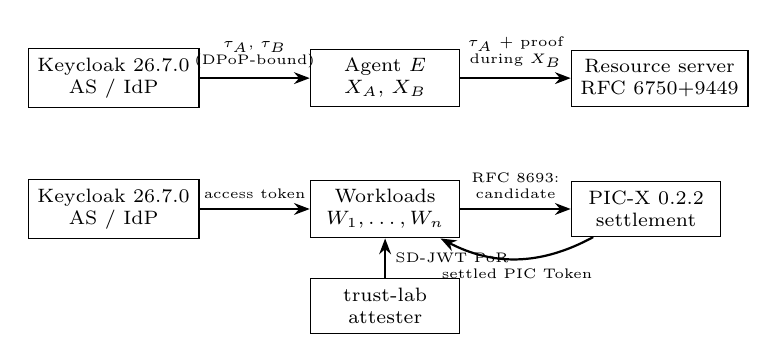
\begin{tikzpicture}[
  box/.style={draw, rectangle, minimum height=7mm, minimum width=19mm, font=\scriptsize, align=center},
  lbl/.style={font=\tiny, align=center},
  arr/.style={-{Stealth[length=2mm]}, thick},
  node distance=6mm and 9mm
]
\node[box] (kc) {Keycloak 26.7.0\\AS / IdP};
\node[box, right=14mm of kc] (agent) {Agent $E$\\$X_A$, $X_B$};
\node[box, right=14mm of agent] (rs) {Resource server\\RFC 6750+9449};
\draw[arr] (kc) -- node[lbl, above] {$\tau_A$, $\tau_B$\\(DPoP-bound)} (agent);
\draw[arr] (agent) -- node[lbl, above] {$\tau_A$ + proof\\during $X_B$} (rs);

\node[box, below=9mm of kc] (kc2) {Keycloak 26.7.0\\AS / IdP};
\node[box, right=14mm of kc2] (agent2) {Workloads\\$W_1,\dots,W_n$};
\node[box, right=14mm of agent2] (picx) {PIC-X 0.2.2\\settlement};
\node[box, below=5mm of agent2] (tl) {trust-lab\\attester};
\draw[arr] (kc2) -- node[lbl, above] {access token} (agent2);
\draw[arr] (agent2) -- node[lbl, above] {RFC 8693:\\candidate} (picx);
\draw[arr] (picx) to[bend left=28] node[lbl, below] {settled PIC Token} (agent2);
\draw[arr] (tl) -- node[lbl, right] {SD-JWT PoR} (agent2);
\end{tikzpicture}
\caption{Testbed. Top: the baseline path (Theorem~\ref{thm:gap}). Bottom: the PIC-X path; the initial RFC~8693 exchange presents the access token and PIC-X mints $\mathrm{PCA}_0$; each later exchange presents a workload-signed candidate and PIC-X settles the next checkpoint.}
\label{fig:testbed}
\end{figure}

\emph{Correspondence to the model.} PIC-X is the Tier-1 remedy of \S\ref{sec:comparison} implemented: an RFC~8693 authorization server that became a continuity verifier. The conjuncts of Def.~\ref{def:acceptpic} map to implemented checks as follows. $\PoR$: the SD-JWT attestation is validated against the configured attester's keys, and the transition, candidate continuity, and candidate token signatures are verified under the key it binds (\texttt{cnf.jwk}). Predecessor binding: the presented checkpoint must be realm-signed, its digest must equal the transition's \texttt{predecessor.hash}, the position must advance by one, and the transition must answer the checkpoint's challenge. $\subseteq$: attenuation is removal-only in the wire format, and non-expansion is checked at settlement; a union state is not expressible as an attenuation of either lineage. $\kappa$: every execution-contract entry of the checkpoint must be disclosed by the attestation and agree with it. $\mathrm{Fresh}$: challenge continuity plus the lineage expiry, which advancement cannot extend. $\neg\mathrm{Revoked}$: not implemented at this commit (Appendix~A); the conjunct is vacuously true in the deployment measured here. Two elements of Def.~\ref{def:por} are profile-conditional and are not exercised: the request digest $\Hsh(q)$ is carried by the wire format but not required by this deployment's policy, and $\mathrm{PCA}_0$ commits to $\rho(X)$ procedurally---PIC-X verifies the access token and mints a fresh lineage identity in the same exchange---rather than by carrying a digest of it. Two further facts about the realization bound what the runs can show: the exchange accepts \emph{bearer} subject tokens (no $\mathrm{cnf}$/DPoP check, \S\ref{sec:oauth} point~4), and downstream receivers of settled tokens discharge the conjuncts by verifying the settlement authority's signatures rather than by re-running them (A2 at that authority, \S\ref{sec:pic}).

\subsection{Runs and observations}

Table~\ref{tab:runs} lists every run. Fixed inputs, scripted, repeatable; Expected is what the paper's statements predict, Observed is the recorded output.

Runs P1--P3 exercise misattribution at the artifact level: the presentations an executor could assemble against the verifier, run to show that each conjunct is live and is named on failure. The application-level counterpart of B1 is run P8: the executor honestly advances lineage $A$ and presents its settled token while serving the workflow that request $B$ started. It is accepted---as a continuation of $X_A$, which is what Def.~\ref{def:validcont} prescribes. Non-mixing \emph{attributes} that write; it does not prevent it. Run P9 is what the attribution buys: the receiver binds the workflow to the lineage of its first presentation and rejects the same save because it continues the wrong occurrence. That policy reads the occurrence carried by the settled token; no baseline receiver can express it, because no baseline input carries an occurrence (Lemma~\ref{lem:invariance})---it is the general form of~\cite[Thm.~4]{gallo2026poc} enforced at a receiving boundary. Run P10 bounds the claim from the other side: individuation is an origination decision (\S\ref{sec:oauth}), and a lineage that origination did not split cannot be split by any receiver.

\begin{table*}[!tp]
\centering
\caption{Runs. Baseline: Keycloak-issued DPoP-bound tokens $\tau_A$ (\texttt{storage.write}) and $\tau_B$ (\texttt{documents.read}) for one principal; the resource server checks all of $T_B$. PIC-X: one grant, two occurrences; lineage $A$ attenuated to $\{\texttt{storage:save}\}$, lineage $B$ to $\{\texttt{documents:read}\}$. Observed values are verbatim from the recorded runs.}
\label{tab:runs}
\small
\begin{tabular}{@{}l>{\raggedright\arraybackslash}p{5.2cm}>{\raggedright\arraybackslash}p{3.6cm}>{\raggedright\arraybackslash}p{5.6cm}@{}}
\toprule
\textbf{Run} & \textbf{Move} & \textbf{Expected} & \textbf{Observed} \\
\midrule
B0 & Correct pairing: $\tau_A$ for $X_A$'s write, $\tau_B$ for $X_B$'s read & Both accepted & \texttt{200} and \texttt{200}; all checks pass \\
B1 & While processing $X_B$, present $\tau_A$ with a fresh valid DPoP proof for a write (Thm.~\ref{thm:gap}) & Accepted; every check passes & \texttt{200}; 17 of 17 receiver checks pass, none failed \\
B1b & Shared accumulator; interleaving \emph{receive A, receive B, execute B, execute A} & Accepted without injected fault & \texttt{200}; the write inside $X_B$ used $\tau_A$ \\
B2 & Same move, executor asserts $\mathrm{exec\_id}=\mathrm{id}(X_B)$; receiver checks it & Accepted (Lemma~\ref{lem:selfasserted}) & \texttt{200}; the check passed on a presenter-chosen value \\
\midrule
P0 & Two lineages from one grant; one further valid continuation each & All accepted & All settlements answered \texttt{200} \\
P1 & Candidate presents $\mathrm{PCA}_A$ (write) while \texttt{predecessor.hash} and challenge answer $\mathrm{PCA}_B$ & Rejected; predecessor binding named & \texttt{400}: ``predecessor.hash does not match the trusted checkpoint bytes'' \\
P2 & Candidate on $\mathrm{PCA}_A$ answering $\mathrm{PCA}_B$'s challenge & Rejected; challenge continuity named & \texttt{400}: ``previous\_challenge does not match the checkpoint next\_challenge'' \\
P3 & Workload-signed checkpoint carrying $C_A\cup C_B$, wrapped in a well-formed candidate (Cor.~\ref{cor:mixing}) & Rejected at settlement and downstream & \texttt{400}: ``root.pca is not the currently trusted checkpoint''; ordinary verifier also rejects; the genuine settled token verifies \\
P3b & Otherwise-valid candidate whose remove bitmap references nonexistent index 5 & Rejected; attenuation validation named & \texttt{400}: ``remove bitmap references a nonexistent index in section invariants'' \\
P4 & Carol, key created after origination, attestation satisfying $\kappa$, advances lineage $B$ (T4) & Accepted & \texttt{200}; settled to position 2 \\
P5 & Same with attestation disclosing \texttt{department=marketing} against a contract requiring \texttt{sensitive-documents} & Rejected; $\kappa$ named & \texttt{400}: ``executor evidence / execution-contract conformance rejected'' \\
P6 & The same checkpoint advanced twice by two workload keys (at-least-once delivery, Prop.~\ref{prop:dup}) & Both accepted; $\mathbf{U}$ not established & Both \texttt{200}; two settled successors, both position 2, same lineage identifier \\
P7 & Lineage and executor revocation & Omitted & Not implemented at commit \texttt{1b485cd}: the realm wires a revocation check that always answers false \\
P8 & While serving the workflow started by $X_B$, present lineage $A$'s settled token for a save; ordinary verification and authority coverage, no occurrence policy & Accepted as a continuation of $X_A$ (Def.~\ref{def:validcont}): attribution, not prevention & Both presentations accepted; the save is accepted naming lineage $A$ \\
P9 & Same two presentations; the receiver binds the workflow to the lineage of its first presentation & Read accepted and binds the workflow to $B$; the save under $A$ rejected by the occurrence policy & Read accepted, workflow bound to lineage $B$; save rejected: ``workflow is bound to lineage $B$; the presentation continues lineage $A$'' \\
P10 & One initial exchange; both application requests served under the one lineage, which carries both invariants & Both accepted: individuation happened at origination, at the executor's choice (\S\ref{sec:oauth}) & Both accepted under the single lineage \\
\bottomrule
\end{tabular}
\end{table*}

Two facts about the mix are not runs but properties of the artifacts, verified in code. First, the transition grammar has no authority-adding operation: attenuations are removal bitmaps plus contract additions that only constrain, so run~P3's union can be presented only as a forged checkpoint, never as an attenuation of either lineage. Second, the two baseline occurrences and the two PIC lineages descend from the same grant of the same principal; nothing in any run forges, expands, or replays an artifact.

The union in P3 is rejected for the trust reason (the checkpoint is not realm-signed), which is reached before non-expansion could be evaluated; the receiving predicate is a conjunction and the first failing conjunct is reported. The Corollary's $\subseteq$ branch is enforced structurally: non-expansion holds by construction of the removal-only materialization, is re-checked at settlement under the attenuation order, and the settlement-side attenuation validation is live---run P3b reaches it with a hand-assembled candidate the Prover's own check would refuse to build, and it rejects naming the invalid bitmap. Forgery is the only way left to present the union, and P3 is that way, rejected.

On B2: we found no supported configuration of Keycloak 26.7.0 by which a client-chosen execution identifier is copied into an exchanged token, so the AS-copied variant of Lemma~\ref{lem:selfasserted} was not exercised on the stock AS; run B2 exercises the receiver-side variant, in which the receiver checks an asserted identifier that the presenter chose. Both variants fail for the same reason: the value is not bound by evidence to the occurrence.

On P4/P5: what these runs establish is that the conformance conjunct is enforced against attester-signed claims---eligibility ($\kappa$ satisfied) and ineligibility ($\kappa$ contradicted) are decided by the disclosed credential, not by the workload's say-so. They do not establish that the attestation is trustworthy: the laboratory attester issues to any caller, and A3 is assumed throughout (\S\ref{sec:threat}).

\subsection{Log excerpts}

Run B1, receiver checks on the mixed presentation (verbatim, trimmed to the check list):

\begin{center}
\scriptsize
\begin{tabular}{@{}ll@{}}
\toprule
\textbf{Check} & \textbf{Result} \\
\midrule
authorization scheme is DPoP (RFC 9449 \S7.1) & pass \\
token kid resolves to an AS-published key & pass \\
token signature verifies (RS256, AS JWKS) & pass \\
iss == \{AS realm\} & pass \\
exp in the future (RFC 7519 \S4.1.4) & pass \\
aud contains baseline-rs (RFC 8707) & pass \\
scope covers the operation (storage.write) & pass \\
token carries cnf.jkt (DPoP-bound, RFC 9449 \S6.1) & pass \\
DPoP header present (RFC 9449 \S4.1) & pass \\
proof typ == dpop+jwt and alg == ES256 & pass \\
proof key thumbprint == cnf.jkt (\S4.3 step 12) & pass \\
proof signature verifies under its own key & pass \\
htm == request method (\S4.3 step 8) & pass \\
htu == request URI (\S4.3 step 9) & pass \\
iat within acceptance window (\S4.3 step 10) & pass \\
jti fresh (\S11.1 replay store) & pass \\
ath == SHA-256(access token) (\S4.3 step 12) & pass \\
\bottomrule
\end{tabular}
\end{center}

Nothing failed: the write that $X_B$ never authorized was performed by a receiver that verified everything RFC~6750 and RFC~9449 direct it to verify. That is Theorem~\ref{thm:gap}'s word \emph{conformant}, observed.

Run P1, the same move under $\Accept_{\mathrm{PIC}}$, settlement response and server-side record (verbatim):

\begin{quote}
\scriptsize
\texttt{HTTP 400 \{"error": "invalid\_grant", "error\_description": "the candidate was rejected: predecessor.hash does not match the trusted checkpoint bytes"\}}

\texttt{\{"level":"WARN", "message":"a candidate PIC Token JWT was rejected", "event.name":"token\_exchange.advancement\_rejected", "realm":"acme", "error":"predecessor.hash does not match the trusted checkpoint bytes"\}}
\end{quote}

\subsection{Performance}

Table~\ref{tab:perf} reports the exchange round trips, all measured by the same client over HTTP on loopback, $N{=}100$ each, and the in-process receiver-side verification costs, $N{=}2000$. The lineage advanced in the measurement reached position~100; the settled token stayed at 1{,}965~bytes, since the centralized profile transports a constant-size checkpoint rather than a growing chain, and one advancement costs the same at position~100 as at position~1.

\begin{table}[!tp]
\centering
\caption{Measurements. Round trips over loopback HTTP ($N{=}100$); verification in-process ($N{=}2000$), Rust, release build.}
\label{tab:perf}
\small
\begin{tabular}{@{}lrr@{}}
\toprule
Exchange round trip & median & p95 \\
\midrule
Keycloak password grant (context) & 19.9 ms & 21.7 ms \\
Keycloak RFC 8693 token exchange & 3.9 ms & 4.7 ms \\
PIC-X initial exchange ($\mathrm{PCA}_0$) & 1.2 ms & 1.7 ms \\
PIC-X advancement (settle candidate) & 2.0 ms & 2.4 ms \\
\midrule
Receiver-side verification (in-process) & \multicolumn{2}{r}{mean} \\
\midrule
Baseline access token, RS256 JWS verify & \multicolumn{2}{r}{10.8 $\mu$s} \\
Baseline DPoP proof, ES256 JWS verify & \multicolumn{2}{r}{27.8 $\mu$s} \\
PIC settled token, ordinary verifier (ES256) & \multicolumn{2}{r}{489.1 $\mu$s} \\
\midrule
Artifact sizes & \multicolumn{2}{r}{bytes} \\
\midrule
OAuth access token & \multicolumn{2}{r}{1{,}246} \\
PIC Token JWT ($\mathrm{PCA}_0$) & \multicolumn{2}{r}{2{,}024} \\
Candidate PIC Token JWT (with PoR) & \multicolumn{2}{r}{3{,}964} \\
Settled PIC Token JWT (position 1 / 100) & \multicolumn{2}{r}{1{,}964 / 1{,}965} \\
\bottomrule
\end{tabular}
\end{table}

The exchange rows are context, not a comparison: Keycloak (Java, database-backed) and PIC-X (Rust, in-memory) are different codebases doing different work, and no ratio between them is a statement about the protocols; the rows establish only that a settlement hop---one SD-JWT validation, three signature verifications, the checks of Def.~\ref{def:acceptpic}, three signatures---completed in 2.0~ms median on this deployment, the same order as the exchanges around it. The one ratio the harness supports is receiver-side, same process, same machine, same language: ordinary verification of a settled token costs 489~$\mu$s against 38.6~$\mu$s for the baseline receiver's two signature checks (RS256 token + ES256 proof), a factor of 12.7, because the settled artifact carries three nested ES256 signatures (token, continuity, checkpoint) plus hashing and CBOR decoding. Both costs are constant in the hop count. The client-side work per hop---obtaining a PoR credential and signing the candidate---measured 0.9~ms and 2.3~ms median respectively, the latter dominated by process-spawn overhead of the harness. These figures are from one warm loopback deployment and carry no claim beyond this machine; the incremental-profile caveat of \S\ref{sec:pic} applies in its centralized form, A2 at the settlement authority.

\subsection{Threats to validity}

The testbed shows receiving rules, not a production system. Conformance of the AS is by a stock Keycloak deployment and conformance of the baseline resource server is by construction against the RFC check lists, not by certification; a certified implementation could differ in checks we did not model, though any such check would still read only $T_B$ and Lemma~\ref{lem:invariance} would apply to it. The attestation issuer is a laboratory service that issues to any caller; A3 is assumed, not tested, and nothing here validates real attestation infrastructure. All traffic is loopback HTTP on one machine: latencies exclude network and TLS, and the comparison between Keycloak and PIC-X round trips compares two different codebases doing different work, not one protocol against another. Revocation, composition, receiver-side full-chain and snapshot validation, and request-digest binding are not implemented at the evaluated commit and are accordingly absent from every claim (Appendix~A). Taken one at a time each omission is declared; taken together they compound: open continuation with no uniqueness supply, no revocation, and an attester that issues to any caller means that, in this deployment as tested, any party that observes a checkpoint and can obtain a laboratory attestation can continue the lineage, repeatedly, until the lineage expires. A production deployment closes that combination with real attestation issuance, revocation, and one of the $\mathbf{U}$ supplies of Prop.~\ref{prop:dup}; none of the three is demonstrated here. The exchange likewise accepts bearer subject tokens, so at the origination seam the PIC path as deployed is weaker than the DPoP-verifying baseline receiver against subject-token theft (\S\ref{sec:oauth} point~4). The duplicate-delivery run redelivers explicitly rather than through a broker; at-least-once semantics is the delivery contract being modeled, and a broker would add no check to either receiving rule.

\section{Related Work}\label{sec:related}

\emph{Capabilities.} Dennis and Van Horn~\cite{dennis1966}, Miller~\cite{miller2003,miller2006}, and Spiessens~\cite{spiessens2007} address the classical confused deputy~\cite{hardy1988} by fusing designation and authority at invocation. Spiessens states the residual dependency explicitly: the capability approach must ``rely upon the deputy not to use'' its own authority in place of the client's~\cite[p.~189]{spiessens2007}. That reliance is what T2 forbids; PIC turns it into a receiver check. Object capabilities remain the answer to designation, which PIC lacks.

\emph{Attenuation chains.} Macaroons~\cite{macaroons} chain HMACs over caveats so that holders can only restrict; Biscuit~\cite{biscuit} does the same with public-key blocks and Datalog checks. Both individuate occurrences if and only if a request-binding caveat or check is present; the specifications do not require it, and neither attests the executor that appended a restriction. UCAN~\cite{ucan} chains delegations between named DIDs with content-addressed proofs and native fan-in; SPKI/SDSI~\cite{rfc2693} reduces certificate chains by intersection with a delegation-control bit. Both name the delegate, which forecloses T4. The distinction this paper draws---\emph{a delegation chain is provenance; it is not an execution lineage}---is what separates all four from continuity.

\emph{OAuth propagation.} Bearer tokens~\cite{rfc6749,rfc6750}, DPoP~\cite{rfc9449}, resource indicators~\cite{rfc8707}, and token exchange with \texttt{act} chains~\cite{rfc8693} establish presenter, audience, and delegation history. Lemma~\ref{lem:invariance} shows that none of their receiver inputs is bound to the occurrence. Rich Authorization Requests~\cite{rfc9396} supply structured consent that \S\ref{sec:oauth} reuses.

\emph{History, provenance, and flow.} History-based access control~\cite{abadi2003} conditions on the code that executed; provenance-based access control~\cite{park2012} on the derivation of data; DIFC~\cite{myers1997} on labels attached to information. PIC conditions on the lineage of authority; a deployment may need all of them.

\emph{Prior model.} The abstract PIC model, the lineage-invariance theorems, and the trade-off theorem are in~\cite{gallo2026poc}. This paper adds the occurrence/provenance/input separation, the field-level invariance lemma for the concrete baseline, the self-asserted-discriminator lemma, the complement equation of Def.~\ref{def:acceptpic}, explicit treatment of $\mathbf{U}$, the three-tier comparison, and the experimental demonstration of \S\ref{sec:impl}.

\section{Limitations}\label{sec:limits}

\emph{Designation.} PIC tracks where authority comes from, not where a target name comes from. A deputy holding housekeeping authority over a namespace can perform a request-designated write within that namespace under its own lineage, and the receiver has no object that says the target was designated by the request. Closing this requires binding payload-derived designations to the request's lineage---a taint from payload to authority---which in turn requires the receiver to interpret payload semantics ($T$). We leave it open and, accordingly, claim only the temporal condition of Def.~\ref{def:tcd}.

\emph{Linear core.} Fork, join, and DAG-shaped executions generalize $\ell$ to a partial order; the sufficiency theorem is proved for chains. Fan-out and $\mathbf{U}$ are addressed by profiles whose semantics must be cited, not assumed.

\emph{Runtime evidence.} The authenticity of evidence evaluated at commit is an input to the guardrail, not a consequence of the model.

\emph{Translation.} Across heterogeneous operation spaces safety is relative to the soundness of $T$; an over-permissive translation is a policy error the invariant cannot detect.

\emph{Origination and attestation.} A4 and A3 are trust boundaries. PIC narrows the trust base to origin, attestation issuers, and verifiers; it does not remove it.

\emph{Origination granularity.} The model individuates occurrences at origination; nothing downstream can split a lineage that origination minted as one. When the party requesting the initial exchange is the executor itself, the granularity of individuation is chosen by the very party the threat model declines to trust (run P10 of \S\ref{sec:impl}). Discharging A4 therefore includes one lineage per origination request, enforced by the originator (\S\ref{sec:oauth} point~6); the evaluated implementation does not yet enforce it.

\emph{Flow.} Exfiltration of data through authorized operations is outside the model.

\emph{Verification status.} Type-checking of the abstract development establishes that the proof terms are accepted; it does not establish A5, adequacy of the model for a deployment, or conformance of an implementation. The experiment of \S\ref{sec:impl} establishes that one implementation rejects the tested mixes and accepts the tested continuations; it is not a conformance proof.

\section{Conclusion}\label{sec:conclusion}

Starting from the strongest token-based propagation stack current specifications support, we showed that a conformant receiver reads no input bound to the execution occurrence it is serving, so authority from one concurrent execution can be accepted as the continuation of another without any participant deviating from specification; that asserting an execution identifier does not help, because assertion is not evidence; and that adding one conjunct---receiver-verifiable binding to the specific predecessor and signed request, with non-expansion---establishes execution-context non-mixing under stated assumptions. Both halves were then executed: a stock authorization server and a receiver checking every field of the strongest baseline accepted the mixed presentation with nothing failing; an implementation of the added conjunct rejected every misattributed presentation naming the failed check, accepted the same authority under its own occurrence, and made that attribution available to a receiver policy---a workflow bound to its lineage---that no execution-invariant receiver can express. Provenance is not continuity. Attenuation-chain systems can supply continuity as a deployment choice; token exchange cannot without becoming a continuity verifier; PIC makes it a protocol invariant. What PIC does not do---designation, information flow, DAG composition, uniqueness of continuation, semantic intent---is stated so that the property it does establish can be relied upon exactly as far as it reaches.

\appendices

\section{PIC-X Capability Inventory}\label{app:inventory}

Table~\ref{tab:inventory} records what PIC-X implements at the evaluated commit, established by reading the source; file references are relative to the repository root~\cite{picx}, commit \texttt{1b485cd}, protocol crate \texttt{pic-protocol}~0.2.3. Anything listed as not implemented is absent from the experimental claims of \S\ref{sec:impl}.

\begin{table*}[!tp]
\centering
\caption{PIC-X capability inventory at commit \texttt{1b485cd} (v0.2.2).}
\label{tab:inventory}
\small
\begin{tabular}{@{}>{\raggedright\arraybackslash}p{4.1cm}>{\raggedright\arraybackslash}p{8.6cm}>{\raggedright\arraybackslash}p{4.2cm}@{}}
\toprule
\textbf{Question} & \textbf{Answer, from code} & \textbf{Where} \\
\midrule
Who mints $\mathrm{PCA}_0$? & The realm (AS role). The RFC~8693 endpoint accepts \texttt{subject\_token\_type = access\_token} plus an initial continuity proposal, verifies the access token (issuer, audience, algorithm, \texttt{typ}, expiry, signature against the identity provider's published keys), maps it to authority, and mints a realm-signed $\mathrm{PCA}_0$ with a fresh lineage identifier and bootstrap challenge. A4 is discharged by the AS; the first executor does not mint. & \path{crates/pic-x-realm/src/exchange.rs} (\texttt{exchange\_initial}, \texttt{validate\_source\_jwt}) \\
\addlinespace
How is scope mapped to $C_0$? & Per-realm exchange profile: configured claim paths for identity context and scopes; prioritized regular-expression rules emit invariant tuples $(\mathrm{scope},o,\mathrm{type},\mathrm{id})$; \texttt{on\_unmatched\_scope: reject}. This is the translation $T$ at hop~0. & \texttt{exchange.rs} (\texttt{map\_authority}, \texttt{map\_invariants}); realm configuration \\
\addlinespace
Does PIC-X verify DPoP? & No. The exchange validates the access token's signature and claims but performs no \texttt{cnf}/DPoP check: it accepts bearer subject tokens, so at the origination seam this deployment is weaker than a DPoP-verifying baseline receiver against subject-token theft. Holder binding at the PIC layer is the PoR-bound workload key. & \texttt{exchange.rs} (no \texttt{cnf} handling) \\
\addlinespace
One lineage per origination request? & Not enforced. The realm is deliberately stateless; the same subject token may initialize any number of lineages (runs P0, P10), and the party choosing the granularity is the executor. Discharging A4 includes this individuation (\S\ref{sec:oauth} point~6). & \path{crates/pic-x-realm/src/checkpoints.rs} (design note); run P10 \\
\addlinespace
What does a successor sign over? & The workload signs three artifacts with the PoR-bound key: a Transition (\texttt{position}, \texttt{predecessor.hash} = SHA-256 of the exact predecessor PCA bytes, \texttt{challenge\{previous,next\}}, removal-only attenuations, typed \texttt{proof\_of\_relationship}, optional \texttt{request\_digest}, optional executor evidence), a candidate Continuity carrying the exact predecessor PCA bytes and that transition, and a candidate PIC Token JWT. The successor $\mathrm{PCA}_{i+1}$ is materialized and signed by the realm at settlement. Differs from an earlier construction sketch in which one artifact carried $\Hsh(q)$ and the attestation directly; the request digest is profile-conditional and unused here. & \texttt{pic-continuity} 0.2.3 (\texttt{prover.rs}, \path{artifacts/transition.rs}); \cite{picspec} Prover/Verifier \S2--3 \\
\addlinespace
What is $\kappa$ and how is it checked? & The execution contract is a key--value section of the checkpoint's authority map. At settlement, every contract entry must be disclosed by the SD-JWT presentation and agree with it; a missing or contradicting disclosure rejects with the conformance reason. The check is against attester-signed claims; the trustworthiness of the attester is A3, assumed and not tested here. & \path{crates/pic-x-realm/src/conformance.rs} \\
\addlinespace
Validation profiles & Centralized settlement (the realm verifies every advancement and issues realm-signed checkpoints); ordinary downstream verification of a settled token is constant-cost. Receiver-side full-chain and snapshot validation are not implemented. & \texttt{exchange.rs} (\texttt{advance}); \texttt{pic-continuity} (\texttt{verify\_settled}) \\
\addlinespace
Replay store / branch profile ($\mathbf{U}$) & None. Checkpoint acceptance is a signature check against the realm's published keys, deliberately stateless; sibling branches from one checkpoint are intentional; challenges are per-lineage, and a transition may not echo the challenge it answers. $\mathbf{U}$ is not provided (run P6). & \path{crates/pic-x-realm/src/checkpoints.rs}; \texttt{exchange.rs} (challenge check) \\
\addlinespace
Revocation & Not implemented: the realm wires a revocation check that always answers false, stated as such in the source. The PIC Revocation specification exists as Draft~0.2. Runs P7/R7 omitted. & \texttt{checkpoints.rs} (\texttt{NoRevocationConfigured}) \\
\addlinespace
Composition / Sandboxed Execution & Not implemented. Specified in~\cite{picsandbox}; no run exercises composition. & --- \\
\addlinespace
Request/execution binding & \texttt{request\_digest} exists in the wire format; the settlement policy hook accepts by default and this deployment does not require it. Not exercised. & \texttt{transition.rs}; \texttt{trust.rs} (\texttt{SettlementPolicy}) \\
\bottomrule
\end{tabular}
\end{table*}

\section{Run Records}\label{app:logs}

Every run of Table~\ref{tab:runs} produced a JSON record (fixed inputs, expected, observed, per-check transcript, timestamps) and a plain-text log; the complete set, together with the one-command testbed (compose file, runner, fault-injection harness), accompanies the paper as an artifact~\cite{picartifact}. Selected verbatim excerpts:

\emph{P2 (challenge splice), settlement response:}
\begin{quote}
\scriptsize
\texttt{HTTP 400 \{"error":"invalid\_grant", "error\_description":"the candidate was rejected: previous\_challenge does not match the checkpoint next\_challenge"\}}
\end{quote}

\emph{P3 (forged union), settlement response and downstream verification:}
\begin{quote}
\scriptsize
\texttt{HTTP 400 \{"error":"invalid\_grant", "error\_description":"the candidate was rejected: root.pca is not the currently trusted checkpoint"\}}

\texttt{ordinary verifier, forged token: rejected (the token is not realm-signed); genuine settled token of lineage A: accepted, position 2, invariants [storage:save]}
\end{quote}

\emph{P5 (contract violation), settlement response:}
\begin{quote}
\scriptsize
\texttt{HTTP 400 \{"error":"invalid\_grant", "error\_description":"the candidate was rejected: executor evidence / execution-contract conformance rejected"\}}
\end{quote}

\emph{P6 (duplicate delivery), observed:}
\begin{quote}
\scriptsize
\texttt{first: accepted, position 2, lineage DgI9u5j0...; second: accepted, position 2, lineage DgI9u5j0...}
\end{quote}

\emph{P3b (invalid attenuation), settlement response:}
\begin{quote}
\scriptsize
\texttt{HTTP 400 \{"error":"invalid\_grant", "error\_description":"the candidate was rejected: remove bitmap references a nonexistent index in section invariants"\}}
\end{quote}

\emph{P9 (occurrence policy at the receiver), check transcript:}
\begin{quote}
\scriptsize
\texttt{step 1 (read, lineage B): settled-token verification: pass; authority covers (read,documents:document-42): pass; workflow `doc-42-pipeline' bound to lineage b5LaF8eg...: pass}

\texttt{step 2 (save, lineage A, inside B's workflow): settled-token verification: pass; authority covers (save,storage:document-42): pass; workflow `doc-42-pipeline' is bound to lineage b5LaF8eg...; the presentation continues lineage p-\_kDadd...: FAIL}
\end{quote}

\emph{P10 (single lineage), observed:}
\begin{quote}
\scriptsize
\texttt{read accepted: True; save accepted: True; both under lineage KU6Qi5QV... --- the receiver cannot separate what origination did not separate}
\end{quote}

\emph{P0/P4 (valid continuations), server-side audit events:} each accepted advancement is recorded before the token is returned, as \texttt{pic.exchange.advanced} with the lineage identifier and position; each rejection as \texttt{token\_exchange.advancement\_rejected} with the failing check named in \texttt{error}.

\begin{thebibliography}{99}

\bibitem{gallo2026poc} N.~Gallo, ``Proof-of-Continuity: A temporal model for authority propagation in distributed systems and AI agents,'' arXiv:2607.08906 [cs.CR], 2026, doi:10.48550/arXiv.2607.08906.

\bibitem{picx} Nitro Agility S.r.l., ``PIC-X: the PIC Authority Broker and Exchange Server,'' v0.2.2, commit \texttt{1b485cd}, \url{https://github.com/pic-protocol/pic-x}; protocol crate \texttt{pic-protocol} 0.2.3, \url{https://crates.io/crates/pic-protocol}.

\bibitem{picspec} Nitro Agility S.r.l., ``PIC Specification, Draft 0.2,'' commit \texttt{5f8703d}, \url{https://github.com/pic-protocol/pic-spec/blob/main/draft/0.2/pic-spec.md}; ``PIC Prover and Verifier Specification, Draft 0.2,'' same repository, \path{draft/0.2/pic-prover-verifier-spec.md}.

\bibitem{picsandbox} Nitro Agility S.r.l., ``PIC Sandboxed Execution, Draft 0.2,'' commit \texttt{5f8703d}, \url{https://github.com/pic-protocol/pic-spec/blob/main/draft/0.2/pic-lineage-guardrail-spec.md}.

\bibitem{picmodellean} N.~Gallo, ``PIC Model: Lean~4 formalization of the Proof-of-Continuity model,'' \url{https://github.com/ngallo/pic-model}, \path{draft/0.1/pic-model-math/pic-lean}, commit \texttt{c02c7db}, Lean \texttt{v4.32.0}.

\bibitem{picartifact} N.~Gallo, ``Experimental artifact for this paper: containerised testbed, run scripts, fault-injection harness, and verbatim run records,'' \url{https://github.com/ngallo/pic-model}, directory \path{draft/0.1/provenance-is-not-continuity}.

\bibitem{rfc6749} D.~Hardt, ``The OAuth 2.0 authorization framework,'' RFC~6749, IETF, 2012.

\bibitem{rfc6750} M.~Jones and D.~Hardt, ``The OAuth 2.0 authorization framework: Bearer token usage,'' RFC~6750, IETF, 2012.

\bibitem{rfc7519} M.~Jones, J.~Bradley, and N.~Sakimura, ``JSON Web Token (JWT),'' RFC~7519, IETF, 2015.

\bibitem{rfc7009} T.~Lodderstedt, S.~Dronia, and M.~Scurtescu, ``OAuth 2.0 token revocation,'' RFC~7009, IETF, 2013.

\bibitem{rfc8693} M.~Jones, A.~Nadalin, B.~Campbell, J.~Bradley, and C.~Mortimore, ``OAuth 2.0 token exchange,'' RFC~8693, IETF, 2020.

\bibitem{rfc8707} B.~Campbell, J.~Bradley, and N.~Sakimura, ``Resource indicators for OAuth 2.0,'' RFC~8707, IETF, 2020.

\bibitem{rfc9396} T.~Lodderstedt, J.~Richer, and B.~Campbell, ``OAuth 2.0 rich authorization requests,'' RFC~9396, IETF, 2023.

\bibitem{rfc9449} D.~Fett, B.~Campbell, J.~Bradley, T.~Lodderstedt, M.~Jones, and D.~Waite, ``OAuth 2.0 demonstrating proof of possession (DPoP),'' RFC~9449, IETF, 2023.

\bibitem{rfc2693} C.~Ellison, B.~Frantz, B.~Lampson, R.~Rivest, B.~Thomas, and T.~Ylonen, ``SPKI certificate theory,'' RFC~2693, IETF, 1999.

\bibitem{hardy1988} N.~Hardy, ``The confused deputy: (or why capabilities might have been invented),'' \emph{ACM SIGOPS Oper. Syst. Rev.}, vol.~22, no.~4, pp.~36--38, 1988.

\bibitem{dennis1966} J.~B. Dennis and E.~C. Van~Horn, ``Programming semantics for multiprogrammed computations,'' \emph{Commun. ACM}, vol.~9, no.~3, pp.~143--155, 1966.

\bibitem{miller2003} M.~S. Miller, K.-P. Yee, and J.~Shapiro, ``Capability myths demolished,'' Tech. Rep. SRL2003-02, Johns Hopkins Univ., 2003.

\bibitem{miller2006} M.~S. Miller, ``Robust composition: Towards a unified approach to access control and concurrency control,'' Ph.D. thesis, Johns Hopkins Univ., 2006.

\bibitem{spiessens2007} A.~Spiessens, ``Patterns of safe collaboration,'' Ph.D. thesis, Universit\'e catholique de Louvain, 2007.

\bibitem{macaroons} A.~Birgisson, J.~G. Politz, \'U.~Erlingsson, A.~Taly, M.~Vrable, and M.~Lentczner, ``Macaroons: Cookies with contextual caveats for decentralized authorization in the cloud,'' in \emph{Proc. NDSS}, 2014.

\bibitem{biscuit} ``Biscuit authorization token, specification v3.3,'' \url{https://github.com/eclipse-biscuit/biscuit} (SPECIFICATIONS.md); \url{https://www.biscuitsec.org}. Accessed 2026-09-05.

\bibitem{ucan} ``UCAN: User Controlled Authorization Networks, specification v1.0.0,'' \url{https://github.com/ucan-wg/spec}; ``UCAN Invocation specification v1.0.0 (optional \texttt{cause} field),'' \url{https://github.com/ucan-wg/invocation}. Accessed 2026-09-05.

\bibitem{abadi2003} M.~Abadi and C.~Fournet, ``Access control based on execution history,'' in \emph{Proc. NDSS}, 2003.

\bibitem{park2012} J.~Park, D.~Nguyen, and R.~Sandhu, ``A provenance-based access control model,'' in \emph{Proc. PST}, 2012, pp.~137--144.

\bibitem{myers1997} A.~C. Myers and B.~Liskov, ``A decentralized model for information flow control,'' \emph{ACM SIGOPS Oper. Syst. Rev.}, vol.~31, no.~5, pp.~129--142, 1997.

\bibitem{denning1976} D.~E. Denning, ``A lattice model of secure information flow,'' \emph{Commun. ACM}, vol.~19, no.~5, pp.~236--243, 1976.

\end{thebibliography}

\end{document}
